%Preámbulo del documento

\documentclass[letterpaper]{article} %Tipo de documento
\usepackage[utf8]{inputenc} % Codificación del texto
\usepackage[spanish]{babel} %Idioma del documento
\usepackage{graphicx} %Inserción de imagenes
\usepackage{amssymb, amsmath} %Fórmulas matemáticas
\usepackage{float}
\usepackage[caption = false]{subfig}
%Cuerpo del documento
\begin{document}
    \begin{figure}[H]
        \begin{titlepage}%Cuerpo de la portada
            
            \centering
            \subfloat{
\includegraphics[width=0.2\textwidth]{unamescudo.png}\par}
            \hspace{7cm}
			\subfloat{
\includegraphics[width=0.2\textwidth]{escudofi_negro}\par}

            \vspace{1cm}
                                    
            \centering
            {\bfseries\LARGE Universidad Nacional Aut\'onoma de M\'exico \par}
            \vspace{1cm}
            {\bfseries\LARGE Facultad de Ingenier\'ia \par}
            \vspace{1cm}
            {\bfseries\LARGE Divisi\'on de Ingenier\'ia El\'ectrica\par}
            \vspace{1cm}
            {\itshape\Large \textbf{Laboratorio de Diseño Digital Moderno\\} \par} 
            \vspace{1cm}
            {\scshape\LARGE{Pr\'actica 2: Lenguaje de descripci\'on de hardware VHDL\\} \par}
            \vspace{1cm}
            {\itshape\Large \textbf{M.I Vicente Flores Olvera\\} \par}
            \vspace{1cm}
            \vfill
            {\itshape\Large Bautista P\'erez Brian Jassiel \\\par}
            {\itshape\Large Serralde Flores Andrea \\\par}
            \vfill
            \vspace{1cm}
            {\itshape\Large \today\par}
            
        \end{titlepage}
	\end{figure}
    \newpage

    \section{1. Objetivo}


    \section*{2. Previo}

    \section*{3. Desarrollo de la pr\'actica}
        \subsection*{3.1. Pr\'actica 2A}
        Programar las funciones mostradas, en un formato SOP y POS m\'inimo (reducido) en
        forma de flujo de datos, para su posterior simulaci\'on dentro de la plataforma Quartus II.

        \begin{equation}
            \label{eq:POS}
            f(xyzt) = (x + \bar{x}y + \overline{yt})(x + (\overline{xy})z)
        \end{equation}

        Funci\'on con formato de Producto de Sumas~\ref{eq:POS}.

        \begin{equation}
            \label{eq:SOP}
            f(uvtw) = vt(u + t\bar{w})(u + \bar{w}) + wu(v +t)
        \end{equation}

        Funci\'on con formato de Suma de Productos~\ref{eq:SOP}.

            \subsection*{3.1.1. Implementaci\'on en Quartus II}

                \begin{figure}[h!]
                    \raggedright
                    \subfloat[Implementaci\'on de las funciones en Quartus II]{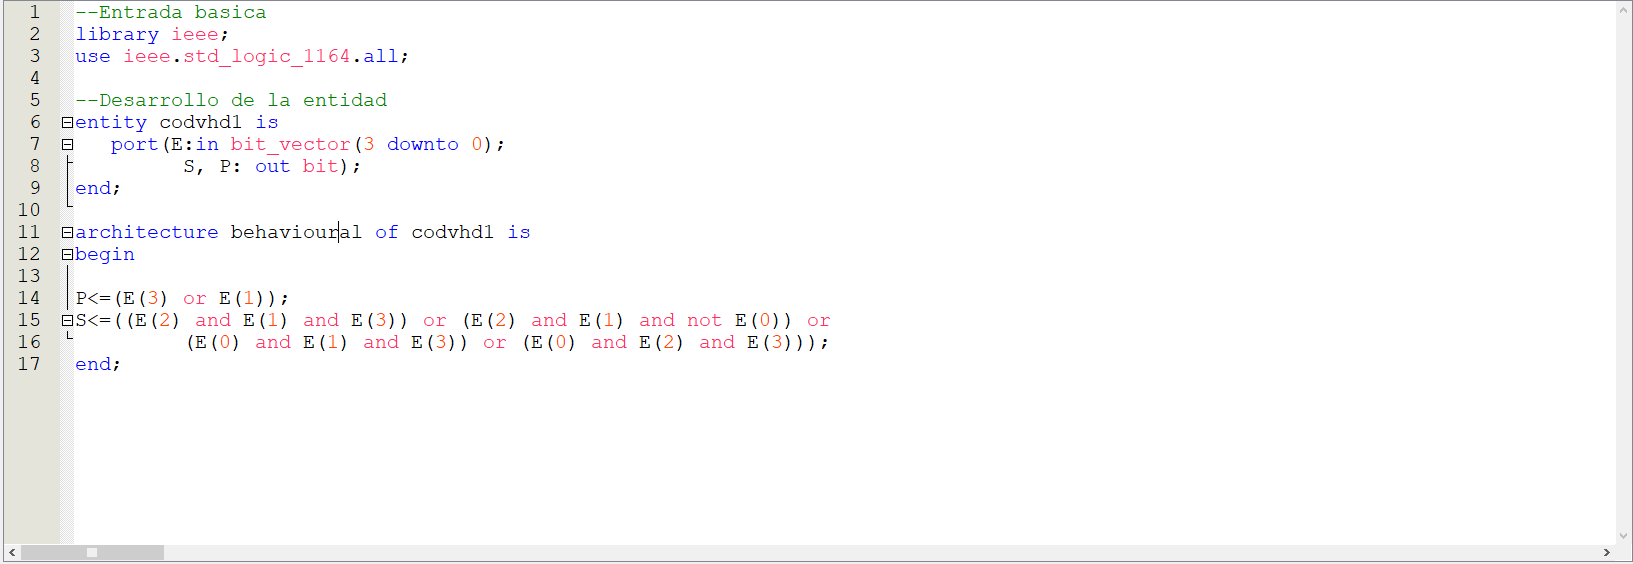
\includegraphics[width = \textwidth]{Codigo1.PNG}}
                \end{figure}


                

                

        \subsection*{3.2. Pr\'actica 2B}
        Programar las funciones expresadas en formato POS Y SOP can\'onicas y m\'inimas del previo
        en forma de flujo de datos, para su posterior simulación dentro de la plataforma Quartus II.

        

    \section*{4. Conclusiones}

    



\end{document}